% !TEX root = ../main.tex

\subsection{Implementation}
shown in \ref{lst:chorus} is the Matlab strip used to generate a course effects.
To test this filter the theme song of monkey Island file in \ref{fig:monkeyIsland}.


\begin{listing}
	\begin{minted}[linenos,breaklines,stepnumber=5,frame=single]{matlab}
%% parameters to vary the effect %
% 3ms max delay in seconds
max_time_delay=0.003;
%rate of flange in Hz
rate=2;                         
%create index array
index=1:length(x_seg);

% Sin reference to create oscillating delay
sin_ref = (sin(2*pi*index*(rate/Fs)))';

%convert delay in ms to max delay in samples
max_samp_delay=round(max_time_delay*Fs);

% create empty out vector
y = zeros(length(x_seg),1);

% to avoid referencing of negative samples
%y(1:max_samp_delay)=x_seg(1:max_samp_delay);

% set gain coefficient
amp=0.7;

% for each sample
for i = (max_samp_delay+1):length(x_seg),
cur_sin=abs(sin_ref(i)); %abs of current sin val 0-1

% generate delay from 1-max_samp_delay and ensure whole number
cur_delay=ceil(cur_sin*max_samp_delay);

% add delayed sample
y(i) = (amp*x_seg(i)) + amp*(x_seg(i-cur_delay));
end
	\end{minted}
	\caption{shows the script used to make the chorus effect}
	\label{lst:chorus}
\end{listing}

\begin{figure}[!hbt]
	\centering
	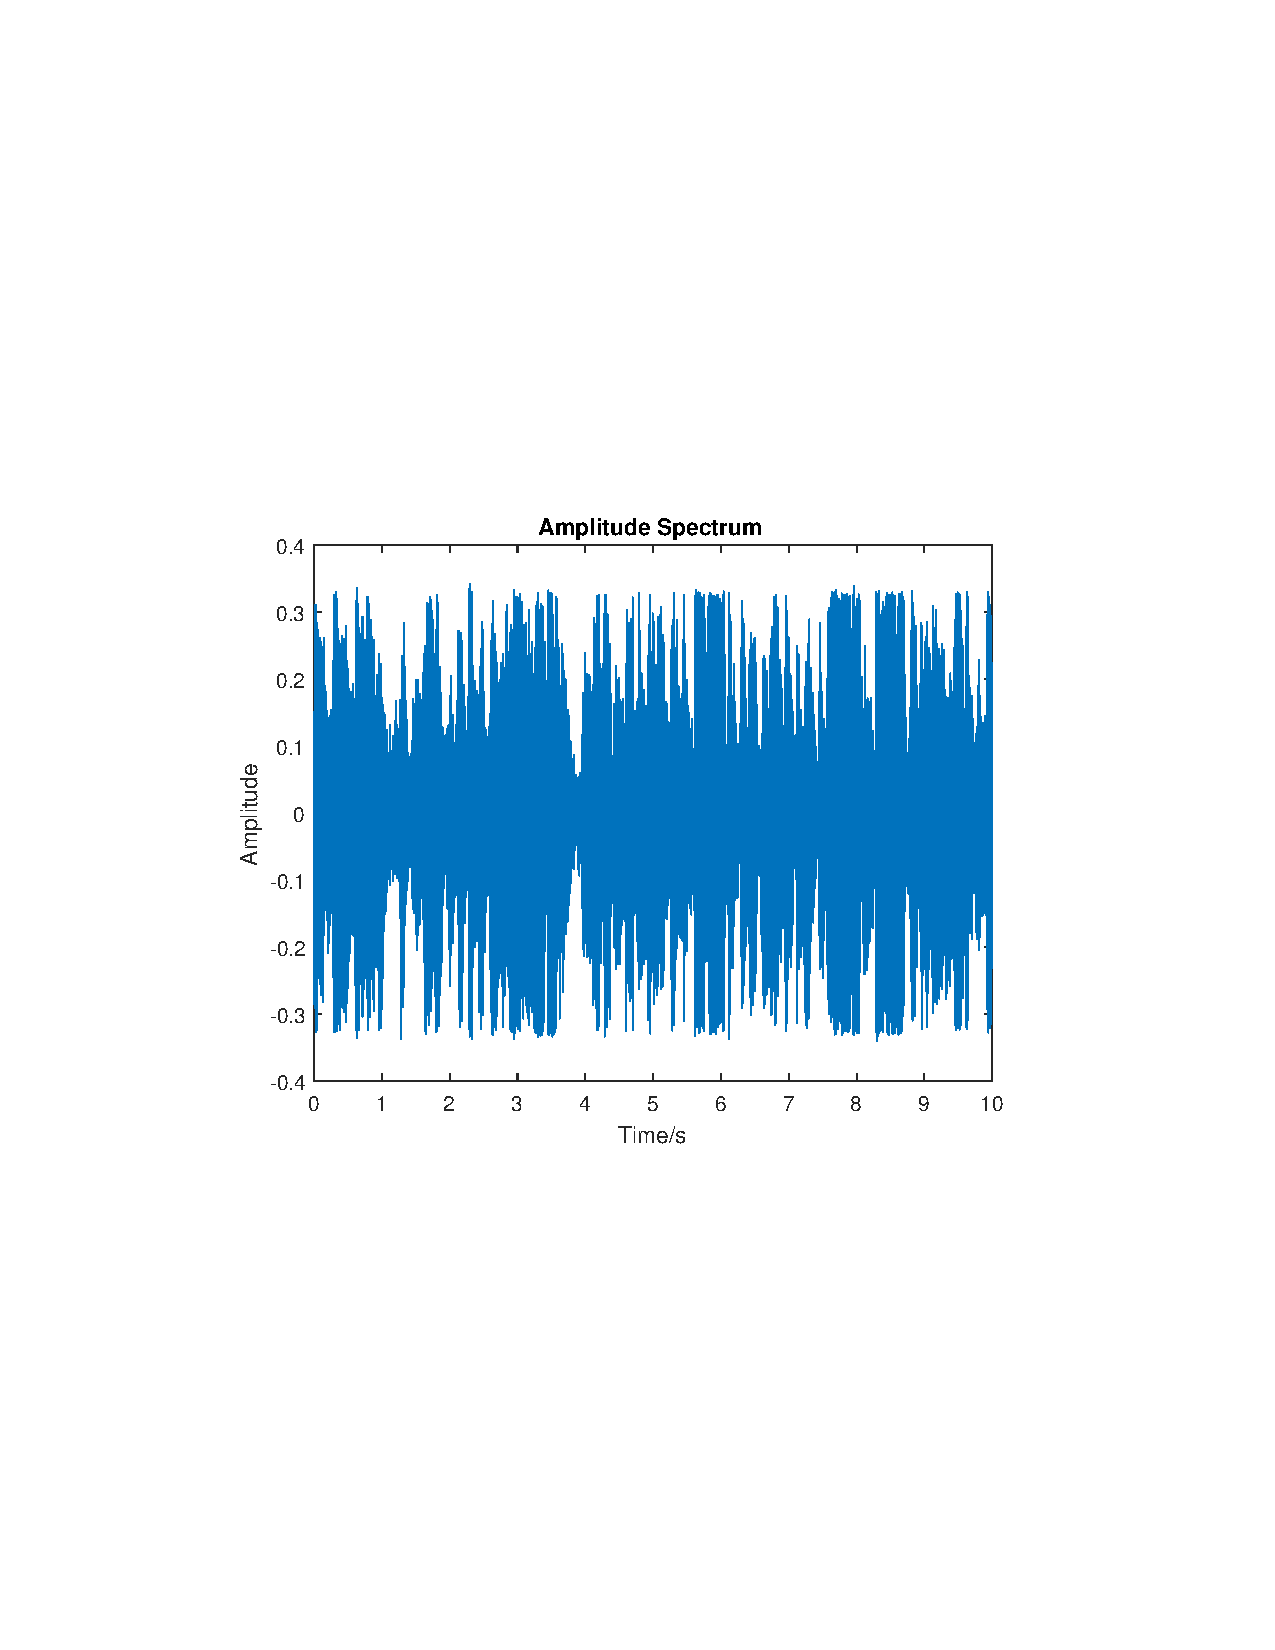
\includegraphics[width=\textwidth]{monkeyIsland.pdf}
	\caption{Excerpt of the theme from Monkey Island in the time domain, without the chorus effect .}
	\label{fig:monkeyIsland}
\end{figure}


